\cleardoublepage
\lgf{\chapter{Experimentons CoAP}}
\lge{\chapter{Let's experiment CoAP}}

\lgf{Les programmes se trouvent dans le répertoire \texttt{pycom} pour l'Objet et \texttt{plido-tp4} pour le serveur.}
\lge{The programs are located in the directory \texttt{pycom} for the Object and \texttt{plido-tp4} for the server.}


\lgf{Les programmes pour l'Objet pourront tourner indifféremment dans une fenêtre de votre ordinateur ou sur votre Pycom. Dans la suite, nous supposerons qu'il s'agit d'une deuxième fenêtre de terminal sur votre ordinateur mais libre à vous de le lancer sur votre Pycom en Wi-Fi (voire en LoRaWAN) pour plus de réalisme. L'utilisation du réseau Sigfox est plus problématique vu que les requêtes provenant de votre Pycom sont limitées à 12 caractères et que les réponses ne sont qu'au nombre de 4 par jour et limitées à 8 caractères. }
\lge{The programs for the Object can run either in a window on your computer or on your Pycom. In the following, we will assume that it is a second terminal window on your computer but feel free to run it on your Pycom in Wi-Fi (or even in LoRaWAN) for more realism. The use of the Sigfox network is more problematic since the requests from your Pycom are limited to 12 characters and the answers are only 4 per day and limited to 8 characters. }

\lgf{Pour nous concentrer sur le fonctionnement de CoAP, nous allons tout d'abord expérimenter en local sur notre ordinateur. Nous verrons par la suite comment utiliser le programme \pprog{generic\_relay.py}{plido-tp3}  pour bénéficier des réseaux LPWAN.}
\lge{To concentrate on the functioning of CoAP, we will first experiment locally on our computer. We will then see how to use the program \pprog{generic\_relay.py}{plido-tp3} to benefit from LPWAN networks}.


\lgf{Attention, le serveur ne fonctionne pas directement sous Windows. Vous devez impérativement le faire tourner dans la machine virtuelle.}
\lge{Be careful, the server does not work directly under Windows. You must run it in the virtual machine.}

\lgf{\section{Mise en œuvre du client/serveur}}
\lge{\section{Client/server implementation}}



 \begin{wrapfigure}{r}{3cm}
\Youtube{https://youtu.be/Nieitr19VGg}
\end{wrapfigure}

\lgf{Nous allons mettre en œuvre le protocole CoAP entre deux processus sur votre machine puis, si vous le voulez, vous pourrez le tester sur un LoPy. Côté Objet, nous allons utiliser une mise en œuvre simple mais compacte du protocole pour comprendre son fonctionnement. À l’autre extrémité, nous utiliserons la mise en œuvre \Index{aiocoap} qui est très complète mais beaucoup plus complexe et demandant plus de ressources.}
\lge{We will implement the CoAP protocol between two processes on your machine and then, if you want, you can test it on a LoPy. On the Object side, we will use a simple but compact implementation of the protocol to understand how it works. At the other end, we will use the \Index{aiocoap} implementation which is very complete but much more complex and resource intensive.}

\subsection{aiocoap}

\lgf{Comme son nom l'indique, aiocoap met en œuvre CoAP, avec les modules asynchronous Input/Output, permettant un fort degré de parallélisme. Le programme suivant (\pprog{coap\_basic\_server1.py}{plido-tp4}) donne un exemple d’un serveur simple gérant une seule ressource time :}
\lge{As its name indicates, aiocoap implements CoAP, with asynchronous Input/Output modules, allowing a high degree of parallelism. The following program (\pprog{coap\_basic\_server1.py}{plido-tp4}) gives an example of a simple server managing a single time resource:}


\pythonlst{coap\_basic\_server1.py}

\begin{itemize}
    \item 
        \lgf{Lignes 21 et 22, l’utilisation de \textit{aicoap} se traduit par l’importation des modules qui se trouvent dans le répertoire \texttt{aoicoap}. }
        \lge{Lines 21 and 22, the use of \textit{aicoap} results in the import of the modules which are in the \texttt{aoicoap} directory. }
    \item  
        \lgf{Dans la fonction \texttt{main} le programme~:}
        \lge{In the function \texttt{main} the program:}
    \begin{itemize}
        \item  
           \lgf{cherche son adresse IP fixe (lignes 40 à 42)~;}
           \lge{looks for its fixed IP address (lines 40 to 42);}
        \item   
            \lgf{fixe à la valeur par défaut le numéro de port à la valeur affectée au serveur CoAP (ligne 44)\footnote{L’utilisation d’une adresse IP et non du joker 0.0.0.0 permet de faire tourner le serveur dans un environnement Windows et MAC};}
            \lge{sets the port number to the default value assigned to the CoAP server (line 44)\footnote{The use of an IP address and not the wildcard 0.0.0.0 allows the server to run in a Windows and MAC environment};}
        \item  
             \lgf{ligne 47, La variable \texttt{root} contient l’arbre des ressources. À la ligne suivante, la ressource \texttt{time} est associée à une classe \texttt{TimeResource}.}
             \lge{line 47, the variable \texttt{root} contains the tree of resources. On the next line, the resource \texttt{time} is associated with a class \texttt{TimeResource}.}
        \item  
        \lgf{La méthode~:}
        \lge{The method:}

\begin{termc}[backgroundcolor=\color{palerod}, basicstyle=\ttfamily\tiny, escapechar=@] 
asyncio.Task(aiocoap.Context.create_server_context(root, bind=(ip_addr, port)))
\end{termc}

            \lgf{permet de lier cet arbre de ressource à l’adresse IP et au numéro de port précédemment défini.}
            \lge{allows to link this resource tree to the IP address and port number previously defined.}
        
        \item  
            \lgf{Ligne 55, le serveur est ensuite lancé dans une boucle sans fin.}
            \lge{Line 55, the server is then launched in an endless loop.}
    \end{itemize}

\end{itemize}

         \vspace{1em}


\lgf{Il est plus intéressant de voir le traitement effectué lorsque la ressource est appelée par le serveur. La classe \texttt{TimeResource} dérivant de la classe générique \texttt{aiocoap} \pfunction{aiocoap}{Resource} est utilisée (ligne 24)~:}
\lge{It is more interesting to see the processing done when the resource is called by the server. The class \texttt{TimeResource} derived from the generic class \texttt{aiocoap} \pfunction{aiocoap}{Resource} is used (line 24):}

\begin{termc}[backgroundcolor=\color{palerod}, basicstyle=\ttfamily\small, escapechar=@] 
class TimeResource(resource.Resource):
\end{termc}

\lgf{Pour chaque méthode CoAP, une méthode peut être définie dans cette classe. Dans l’exemple, la méthode \texttt{render\_get} permet de traiter les requêtes GET. }
\lge{For each CoAP method, a method can be defined in this class. In the example, the method \texttt{render\_get} allows to treat the GET requests. }


         \vspace{1em}


\lgf{Pour simuler un temps de traitement, le programme commence par attendre 5 secondes (ligne 27) puis construit la chaîne de caractères contenant la date qu’il va retourner dans un objet \texttt{aoicoap} \pfunction{aoicoap}{Message}.}
\lge{To simulate a processing time, the program starts by waiting for 5 seconds (line 27) and then constructs the string containing the date that it will return in a \texttt{aoicoap} object \pfunction{aoicoap}{Message}.}

         \vspace{1em}


\lgf{Ainsi, si tout se passe correctement, la réponse à une requête (Code = 0x01) sera 2.05 (Content). La figure~\vref{fig-CoAP-date} résume cet échange que nous avions vu théoriquement dans le chapitre~\vref{chap-token} consacré aux tokens.}
\lge{Thus, if everything goes well, the answer to a request (Code = 0x01) will be 2.05 (Content). The figure~\vref{fig-CoAP-date} summarizes this exchange that we had seen theoretically in the chapter~\vref{chap-token} devoted to tokens.}


\begin{figure}
\centering
	\begin{tikzpicture}[scale=1.5, transform shape] 
	
	\draw [drop shadow, color=verttelecom, -fast cap, line width=3pt] (1, 6) coordinate (a) -- (1, 1);
	\draw [drop shadow, color=verttelecom, -fast cap, line width=3pt] (4, 6) coordinate (b) -- (4, 1);
	
	\draw (a) node [above, verttelecom] {\tiny{Client}};
	\draw (b) node [above, verttelecom] {\tiny{Serveur}};
	
		\draw [ultra thick,  color=purple, drop shadow, ->] (1, 5.5) -- node [above, near end, sloped, text width=4cm] {\tiny{CON MID=0x1234\\Token=12\\GET /time\\}} (4, 5); 
		\draw [color=verttelecom, thick] (1, 5.5) -- +(-0.5, 0); 
		\draw [ultra thick,  color=purple, drop shadow, ->] (4, 5) -- node [below, sloped] {\tiny{ACK MID=0x1234}} (1, 4.5); 
		\draw [color=red, -diamond] (0.75, 5.5) -- node [below, sloped] {\tiny{Timer}} +(0, -1); 
		\draw [color=verttelecom, thick] (1, 4.5) -- +(-0.5, 0); 
		\draw [dotted, color=purple, -triangle 60] (4,5) to [bend left=90] (4, 2.5); 
		\draw [ultra thick,  color=purple, drop shadow, ->] (4, 2.5) -- node [above, near start, sloped, text width=4cm] {\tiny{CON MID=0xF00D\\Token=12\\2.05 "2020-09-05 20:15"\\}} (1, 2); 
		\draw [color=verttelecom, thick] (4, 2.5) -- +(0.5, 0); 
		\draw [ultra thick,  color=purple, drop shadow, ->] (1, 2) -- node [below, sloped] {\tiny{ACK MID=0xF00D}} (4, 1.5); 
		\draw [color=red, -diamond] (4.25, 2.5) -- node [above, sloped] {\tiny{Timer}} +(0, -1); 
		\draw [color=verttelecom, thick] (4, 1.5) -- +(0.5, 0); 
	
	\end{tikzpicture}
\lgf{\caption{Récupération de la date} }
\lge{\caption{Date retrieval} }
\label{fig-CoAP-date} 
\end{figure} 	

\lgf{\subsection{côté Objet}}
\lge{\subsection{Object side}}

\lgf{Du coté du client, nous allons utiliser une mise en œuvre plus compacte qui nous permettra d’expérimenter le fonctionnement de CoAP en modifiant les valeurs des champs protocolaires.}
\lge{On the client side, we will use a more compact implementation that will allow us to experiment the operation of CoAP by changing the values of the protocol fields.}


         \vspace{1em}

\pycomlst{coap\_empty\_msg.py}

\lgf{Le programme \lprog{coap\_empty\_msg.py}{pycom} est beaucoup plus simple. Dans un premier temps, vous devez remplacer l’adresse IP par celle fournie par votre serveur CoAP. Le programme crée une socket UDP au travers de laquelle l’échange avec le serveur sera effectué. La première action consiste à créer un message \lfunction{CoAP}{CoAP} (ligne 9) et à  la ligne suivante créer un en-tête obligatoire avec les paramètres par defaut avec la fonction \lprog{CoAP}{new_header}.}
\lge{The program \lprog{coap\_empty\_msg.py}{pycom} is much simpler. First, you must replace the IP address with the one provided by your CoAP server. The program creates a UDP socket through which the exchange with the server will be made. The first action consists in creating a message \lfunction{CoAP}{CoAP} (line 9) and on the next line create a mandatory header with the default parameters with the function \lprog{CoAP}{new_header}.}


\lgf{Le programme affiche le message avec la fonction  \lfunction{CoAP}{dump}(ligne 11) et l’envoie sur la socket. La ligne 13 permet de limiter l’attente de la réponse à 10 secondes. Cette réponse est attendue ligne 16, transformée en message CoAP ligne 17 et affichée.}
\lge{The program displays the message with the function \lfunction{CoAP}{dump}(line 11) and sends it to the socket. Line 13 allows to limit the waiting time of the answer to 10 seconds. This answer is expected on line 16, transformed into a CoAP message on line 17 and displayed.}


         \vspace{1em}

\lgf{Lancez une capture Wireshark pour voir le trafic passant sur le port de CoAP (\texttt{udp.port==5683} dans la fenêtre de filtrage).}
\lge{Run a Wireshark capture to see the traffic passing through the CoAP port (\texttt{udp.port==5683} in the filter window).}

         \vspace{1em}

\lgf{Lancez maintenant le programme client.}
\lge{Now start the client program.}

\begin{termc}[backgroundcolor=\color{gray!10}, basicstyle=\ttfamily\small, escapechar=@] 
b ’ 40000001 ’
CON 0 x0001 EMPTY
b ’ 70000001 ’
RST 0 x0001 EMPTY
\end{termc}

\lgf{Les messages suivants ont circulé sur le réseau.}
\lge{The following messages were circulated on the network.}

\begin{termc}[backgroundcolor=\color{blue!10}, basicstyle=\ttfamily\tiny, ] 
18:38:30.381449 IP 192.168.1.26.50883 > 192.168.1.26.5683: UDP, length 4
	0x0000:  4500 0020 221f 0000 4011 0000 c0a8 011a  E..."...@.......
	0x0010:  c0a8 011a c6c3 1633 000c 83a2 4000 0001  .......3....@...
18:38:30.382107 IP 192.168.1.26.5683 > 192.168.1.26.50883: UDP, length 4
	0x0000:  4500 0020 efbb 0000 4011 0000 c0a8 011a  E.......@.......
	0x0010:  c0a8 011a 1633 c6c3 000c 83a2 7000 0001  .....3......p...
\end{termc}

\lgf{On retrouve dans le contenu des messages UDP, le message CoAP donné par l’application. Si l’on prend le deuxième message, il commence par 0x70 ; ce qui correspond en binaire à \texttt{0b01\_11\_0000}, soit version = 1, type = 3 et longueur du token = 0.
L’octet suivant donne le code 0 (\Index{Empty}) et les deux derniers octets contiennent le message ID. }
\lge{One finds in the contents of the UDP messages, the CoAP message given by the application. If we take the second message, it starts with 0x70; which corresponds in binary to \texttt{0b01\_11\_0000}, that is to say version = 1, type = 3 and length of the token = 0.
The following byte gives the code 0 (\Index{Empty}) and the last two bytes contain the ID message. }

\lgf{Le serveur ne sachant pas quoi faire de la requête, la rejette en envoyant un message ReSeT\index{RST} pour essayer d’arrêter le code sur le client qui envoie ce genre de requête.}
\lge{The server doesn't know what to do with the request, so it rejects it by sending a ReSeT\index{RST} message to try to stop the code on the client that sends this kind of request.}


\section {GET \texttt{/time}}

\lgf{Nous laissons tourner le serveur CoAP et nous allons construire la requête CoAP du client pour qu'il demande la ressource \texttt{/time}\footnote{N'oubliez pas de mettre la bonne adresse IP du SERVER dans ce programme et dans les suivants}.}
\lge{We let the CoAP server run and we are going to build the CoAP request from the client to ask for the resource \texttt{/time}\footnote{Don't forget to put the right IP address of the SERVER in this program and in the following ones}.}


\pycomlst{coap\_get\_time.py}

\lgf{la méthode \pfunction{CoAP}{new\_header} précise le code, ici GET et et on ajoute l'élément d'URI time en option (ligne 10) grâce à la méthode \pfunction{CoAP}{add\_option}. Côté client, on obtient le résultat suivant :}
\lge{the method \pfunction{CoAP}{new\_header} specifies the code, here GET and and we add the URI time element in option (line 10) thanks to the method \pfunction{CoAP}{add\_option}. On the client side, we obtain the following result:}


\begin{termc}[backgroundcolor=\color{gray!10}, basicstyle=\ttfamily\small, escapechar=@] 
> python3 coap_get_time1.py
False
b'40010001b474696d65'
CON  0x0001 GET   
> Uri-path : b'time'
b'60000001'
ACK  0x0001 EMPTY 
\end{termc}

\lgf{La requête CoAP commence par le mot \texttt{40010001}, indiquant un message \Index{CON}firmable, sans Token, un code GET et un MID de 0x0001, suivi de l'option \Index{Uri-Path}.}
\lge{The CoAP request starts with the word \texttt{40010001}, indicating a \Index{CON}firmable message, with no Token, a GET code and a MID of 0x0001, followed by the \Index{Uri-Path} option.}


         \vspace{1em}

\lgf{La réponse est un \Index{ACK} avec la même valeur de  \textit{Message} ID et le code est vide (0.00).}
\lge{The response is an \Index{ACK} with the same value of \textit{Message} ID and the code is empty (0.00).}


         \vspace{1em}

On n'obtient pas la réponse au GET, juste un acquittement. Pourtant, les log du serveur et l'analyse du réseau montrent bien que le serveur à répondu.

\begin{termc}[backgroundcolor=\color{palerod}, basicstyle=\ttfamily\tiny, escapechar=@] 
DEBUG:coap-server:Incoming message <aiocoap.Message at 0x7f3d997ace80: Type.CON GET (MID 1, empty token) remote 
<UDP6EndpointAddress 192.168.1.79:52495 (locally 192.168.1.79%lo)>, 1 option(s)>
DEBUG:coap-server:New unique message received
DEBUG:coap-server:Sending empty ACK: Response took too long to prepare
DEBUG:coap-server:Sending message <aiocoap.Message at 0x7f3d99742748: Type.ACK EMPTY (MID 1, empty token) remote 
<UDP6EndpointAddress 192.168.1.79:52495 (locally 192.168.1.79%lo)>>
\end{termc}

Les trames qui ont circulé sur le réseau sont représentées figure~\vref{fig-get-time1}. Comme nous avons ajouté un délai de 5 secondes avant de répondre sur le serveur CoAP dans la méthode \texttt{render\_get}, le serveur acquitte la requête et cherche 5 secondes plus tard à envoyer une nouvelle requête confirmée. Mais le client, ayant fermé sa socket, ne peut plus la recevoir et retourne une erreur ICMP.

\begin{figure}[tbp]
\centerline{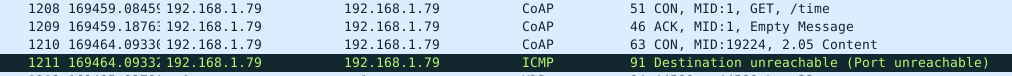
\includegraphics[width=1\columnwidth]{Pictures/get-time1.png}}
\caption{Échange incomplet}
\label{fig-get-time1}
\end{figure}

         \vspace{1em}


La solution est d'attendre un second message et de le décoder comme le montre le listing suivant qui donne le code du programme \lprog{coap\_get\_time2.py}{pycom} dans lequel vous n'aurez pas oublié de changer l'adresse IP du serveur.

\pycomlst{coap\_get\_time2.py}

Nous pouvons laisser éclater notre joie car nous avons la réponse :

\begin{termc}[backgroundcolor=\color{gray!10}, basicstyle=\ttfamily\small, escapechar=@] 
> python3 coap_get_time2.py
False
CON  0x0001 GET   
> Uri-path : b'time'
ACK  0x0001 EMPTY 
CON  0x2708 2.05  
---CONTENT
hex: b'323032312d30332d33302031343a3537'
txt: b'2021-03-30 14:57'
\end{termc}

Mais notre joie est de courte durée car si on regarde plus attentivement la figure~\vref{fig-get-time2} le trafic sur le réseau, on voit que la réponse a été émise deux fois et que l'on retrouve ensuite une erreur ICMP. Cela est dû au fait que l'on n'acquitte pas le message venant du serveur. Le croyant perdu, il le retransmet et tombe sur une socket inexistante. 



\begin{figure}[tbp]
\centerline{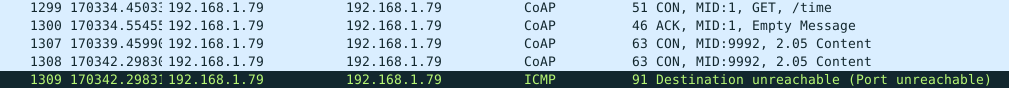
\includegraphics[width=1\columnwidth]{Pictures/get-time2.png}}
\caption{Échange encore incomplet}
\label{fig-get-time2}
\end{figure}

         \vspace{1em}

Pour bien faire, nous devons fournir un acquittement au serveur avec ce code de client avec le programme \lprog{coap\_get\_time3.py}{pycom}.

\pycomlst{coap\_get\_time3.py}

Ici, l'exécution est parfaite :

\begin{termc}[backgroundcolor=\color{gray!10}, basicstyle=\ttfamily\small, escapechar=@] 
> python3 coap_get_time3.py
False
CON  0x0001 GET   
> Uri-path : b'time'
ACK  0x0001 EMPTY 
CON  0x2709 2.05  
---CONTENT
hex: b'323032312d30332d33302031353a3133'
txt: b'2021-03-30 15:13'
ACK  0x2709 EMPTY 
\end{termc}

\noindent si vous n'avez pas oublié de changer l'adresse IP du serveur, et l'utilisation du réseau est optimale (cf figure~\vref{fig-get-time3}).

\begin{figure}[tbp]
\centerline{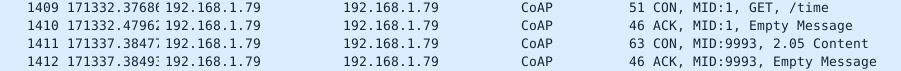
\includegraphics[width=1\columnwidth]{Pictures/get-time3.png}}
\caption{Échange dans les règles de l'art}
\label{fig-get-time3}
\end{figure}

Enfin, on peut ajouter un token pour lier les deux transactions. Ici, il n'y a pas d’ambiguïté car nous ne demandons qu'une seule ressource. Mais si nous demandions plusieurs ressources simultanément, il faudrait pouvoir associer la réponse à la requête. Le programme \lprog{coap\_get\_time4.py}{pycom} ajoute lors de la création de l'en-tête un champ token.

\pycomlst[firstline=9,lastline=12, firstnumber=9]{coap\_get\_time4.py}

L'échange est le même mais le token est répété dans la réponse.

\begin{termc}[backgroundcolor=\color{gray!10}, basicstyle=\ttfamily\small, escapechar=@] 
> python3 coap_get_time4.py
False
CON  0x0001 GET   T=012345
> Uri-path : b'time'
ACK  0x0001 EMPTY 
CON  0x270A 2.05  T=012345
---CONTENT
hex: b'323032312d30332d33302031353a3232'
txt: b'2021-03-30 15:22'
ACK  0x270A EMPTY 
\end{termc}

\Question{NON}
{Que se passe-t-il si vous utilisez une requête non confirmable pour demander la ressource /time (mettre l'argument \texttt{type=CoAP.NON} dans la construction de l'en-tête obligatoire).
 \begin{itemize}[label=$\circ$]
   \item \Wrong{Ça plante le serveur.}
   \item \Wrong{Le serveur répond par une requête Confirmable.}
   \item \Wrong{ Le serveur retourne un RST car nous n'avons pas programmé ce cas.}
   \item \Correct{Le serveur répond par une requête Non Confirmable.}
   \item \Wrong{On passe en heure d'hiver.}
\end{itemize}
}
{}

\Question{Réponse immédiate et CON}{
Modifiez le programme du serveur pour supprimer le délai de 5 secondes avant une réponse.

Que se passe-t-il quand le client envoie une requête CONfirmable ?

 \begin{itemize}[label=$\circ$]
   \item \Correct{Le serveur retourne la réponse dans l'acquittement.}
   \item \Wrong{Le serveur retourne une requête NON confirmable.}
   \item \Wrong{Le serveur attend quand même quelques secondes pour ne pas saturer le réseau.}
   \item \Wrong{Le serveur enlève le token de la réponse..}
\end{itemize}
 }{}
 
 \Question{Réponse immédiate et NON}{
Modifiez le programme du serveur pour supprimer le délai de 5 secondes avant une réponse.

Que se passe-t-il quand le client envoie une requête NON confirmable ?

 \begin{itemize}[label=$\circ$]
   \item \Wrong{Le serveur retourne la réponse dans l'acquittement.}
   \item \Correct{Le serveur retourne une requête NON confirmable.}
   \item \Wrong{Le serveur attend quand même quelques secondes pour ne pas saturer le réseau.}
   \item \Wrong{Le serveur enlève le token de la réponse..}
\end{itemize}
 }{}
 
 
 \section{POST}
 
 \subsection {Ressource codée en ASCII}
 
 Nous allons voir le traitement d’une requête POST avec \textit{aiocoap}. Nous aurions pu ajouter ce traitement à la classe \pfunction{aiocoap}{TimeResource} vue précédemment, mais nous avons préféré ajouter une nouvelle ressource pour le traitement des températures. 

Les lignes suivantes ont été ajoutées pour traiter le POST. Notez le nom de la méthode \texttt{render\_post}.

\pythonlst[firstline=34,lastline=39, firstnumber=34]{coap\_basic\_server2.py}


La réponse à la requête est le code 2.04 (\texttt{aiocoap.CHANGED}) qui indique que la ressource été modifiée. 

On lui associe une nouvelle classe dans l’arbre des ressources :


\pythonnxt[firstline=59,lastline=59, firstnumber=59]{coap\_basic\_server2.py}

Le tout forme le programme \pprog{coap\_basic\_server2.py}{plido-tp4}.

         \vspace{1em}

Coté client, le principe est le même que pour le GET. Dans le programme \lprog{coap\_post\_temp1.py}{pycom}, la méthode \pfunction{CoAP}{add\_payload} permet d’ajouter du contenu à la requête POST. Le programme émet sa requête et affiche le résultat. Nous allons également simplifier la gestion des réponses en utilisant la fonction \pfunction{CoAP}{send\_ack} du module \texttt{CoAP}. Cette fonction prend en argument une socket, un tuple de destination et le message CoAP à envoyer. Elle va le retransmettre au maximum 4 fois tant qu’elle n’a pas reçu l’acquittement correspondant.

\pycomlst{coap\_post\_temp1.py} %[firstline=9,lastline=12, firstnumber=9]

La figure~\vref{fig-duree-max} a montré un échange avec perte. Elles peuvent être simulées en arrêtant le programme serveur sur votre ordinateur.

Lancez le serveur \pprog{coap\_basic\_server2.py}{plido-tp4} et tapez ctrl-Z pour stopper son exécution, tout en laissant ouverte la socket.

\begin{termc}[backgroundcolor=\color{palerod}, basicstyle=\ttfamily\small, escapechar=@] 
> python3 ./coap_basic_server2.py 
server running on  192.168.1.79 at port 5683 ^Z
Job 2, “python3 ./coap_basic_server2.py” has stopped
>
\end{termc}

Lancez le client \lprog{coap\_port\_temp1.py}{pycom} (en n'oubliant pas de changer l'adresse IP du serveur).

\begin{termc}[backgroundcolor=\color{gray!10}, basicstyle=\ttfamily\small, escapechar=@] 
> python3.9 coap_post_temp1.py 
False
CON  0x0001 POST  
> Uri-path : b'temp'
---CONTENT
hex: b'32332e35'
txt: b'23.5'
timeout 2 1
timeout 4 2
\end{termc}

On voit que le client ne reçoit pas l'acquittement, déclenche un temporisateur et retransmet le message. La durée du temporisateur double à chaque tentative\footnote{Le standard recommande d'ajouter un aléa lors de la transmission pour éviter que deux équipements se synchronisent et se perturbent toujours en même temps. Il n'est pas mis en œuvre dans cet exemple.}.

Réactivez le serveur coap en tapant \texttt{fg} (foregroung)

\begin{termc}[backgroundcolor=\color{palerod}, basicstyle=\ttfamily\tiny, escapechar=@] 
> fg
DEBUG:coap-server:Incoming message <aiocoap.Message at 0x7f05d621fcc0: Type.CON POST (MID 1, empty token) remote 
<UDP6EndpointAddress 192.168.1.79:37286 (locally 192.168.1.79%lo)>, 1 option(s), 4 byte(s) payload>
DEBUG:coap-server:New unique message received
--------------------
payload: b'32332e35'
DEBUG:coap-server:Sending message <aiocoap.Message at 0x7f05d622df98: Type.ACK 2.04 Changed (MID 1, empty token) 
remote <UDP6EndpointAddress 192.168.1.79:37286 (locally 192.168.1.79%lo)>>
DEBUG:coap-server:Incoming message <aiocoap.Message at 0x7f05d621fcc0: Type.CON POST (MID 1, empty token) remote 
<UDP6EndpointAddress 192.168.1.79:37286 (locally 192.168.1.79%lo)>, 1 option(s), 4 byte(s) payload>
INFO:coap-server:@\ul{Duplicate CON received, sending old response again}@
DEBUG:coap-server:Sending message <aiocoap.Message at 0x7f05d622df98: Type.ACK 2.04 Changed (MID 1, empty token) 
remote <UDP6EndpointAddress 192.168.1.79:37286 (locally 192.168.1.79%lo)>>
DEBUG:coap-server:Socket error recevied, details: SockExtendedErr(ee_errno=111, ee_origin=2, ee_type=3, ee_code=3, 
ee_pad=0, ee_info=0, ee_data=0)
DEBUG:coap-server:Incoming error 111 from <UDP6EndpointAddress 192.168.1.79:37286 (locally 192.168.1.79%lo)>
DEBUG:coap-server:Incoming message <aiocoap.Message at 0x7f05d622deb8: Type.CON POST (MID 1, empty token) remote 
<UDP6EndpointAddress 192.168.1.79:37286 (locally 192.168.1.79%lo)>, 1 option(s), 4 byte(s) payload>
INFO:coap-server:@\ul{Duplicate CON received, sending old response again}@
DEBUG:coap-server:Sending message <aiocoap.Message at 0x7f05d622df98: Type.ACK 2.04 Changed (MID 1, empty token) 
remote <UDP6EndpointAddress 192.168.1.79:37286 (locally 192.168.1.79%lo)>>
DEBUG:coap-server:Socket error recevied, details: SockExtendedErr(ee_errno=111, ee_origin=2, ee_type=3, ee_code=3, 
ee_pad=0, ee_info=0, ee_data=0)
DEBUG:coap-server:Incoming error 111 from <UDP6EndpointAddress 192.168.1.79:37286 (locally 192.168.1.79%lo)>
\end{termc}

On peut observer plusieurs phénomènes :

\begin{itemize}
    \item le serveur avait gardé en mémoire les requêtes précédentes mais ne les avait pas traitées car le programme avait été stoppé. En le redémarrant, il va pouvoir les traiter. Il répond donc au client qui peut afficher la notification 2.04 ;
    \item les autres requêtes sont vues comme des répétitions de la première puisque le champ Message ID est identique. Le serveur se contente de retourner une copie ;
    \item le client ayant terminé sa transaction a fermé la socket conduisant à l'émission d'un message ICMP qui conduit à l'affichage du message de log d'erreur (Socket error received). 
\end{itemize}

         \vspace{1em}


Ceci peut être vérifié sur la capture Wireshark (cf. figure~\vref{fig-post-ws}).

\begin{figure}[tbp]
\centerline{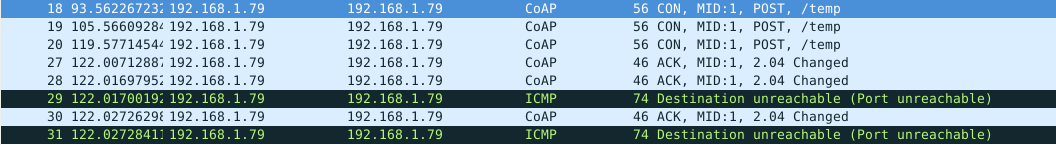
\includegraphics[width=1\columnwidth]{Pictures/coap-ws.png}}
\caption{Trafic lié au POST}
\label{fig-post-ws}
\end{figure}


\subsection{Ressource codée en CBOR}

Le programme précédent, est correct mais nous avons utilisé le format ASCII de transfert par défaut (\textit{\Index{Content-format}} = 0). Il serait préférable de revenir au format JSON ou \Index{CBOR} que nous avions vu précédemment. Pour ce faire, nous devons ajouter dans l’en-tête de la requête l’option Content-format. Comme son code est 12, elle doit être placée après l’option Uri-path (cf. tableau~\vref{tab-CoAP-options}).

\pycomlst{coap\_post\_temp2.py} %[firstline=9,lastline=12, firstnumber=9]

Notez que ce programme,  pprog{coap\_post\_temp2.py}{pycom},  peut aussi bien s'exécuter sur votre ordinateur ou sur votre LoPy. Dans le premier cas, le module \texttt{cbor2} sera utilisé. Sur le LoPy, nous ferons appel au module \texttt{kpn\_senml}. Dans les deux cas, le contenu est transformé en CBOR grâce à la fonction \pfunction{cbor2}{dumps}.

         \vspace{1em}

Du coté du serveur, la méthode\texttt{render\_post} doit connaître le format de la ressource. Pour ce faire, elle doit accéder aux options CoAP.

\pythonlst[firstline=34,lastline=50, firstnumber=34]{coap\_basic\_server3.py} %

Dans le programme \pprog{coap\_basic\_server3.py}{plido-tp4}, la variable \texttt{ct} contient la valeur de l’option \Index{Content-format} si elle existe. De manière générale, \textit{aiocoap} permet d’accéder aux valeurs de toutes les options CoAP contenues dans la requête. La valeur \texttt{None} indique que l’option n’est pas présente dans l’en-tête. Dans ce cas, la variable \texttt{ct} contiendra la valeur par défaut indiquant un texte en ASCII.

Suivant le format de la donnée, le programme affichera le texte ou le CBOR transformé en chaîne de caractères avec la fonction \pfunction{cbor2}{loads}. Si le format n’est pas connu du programme, un code d’erreur est retourné au client.

         \vspace{1em}

La figure~\vref{fig-post2-ws} montre l'échange lié au POST et détaille contenu de la requête.

\begin{figure}[tbp]
\centerline{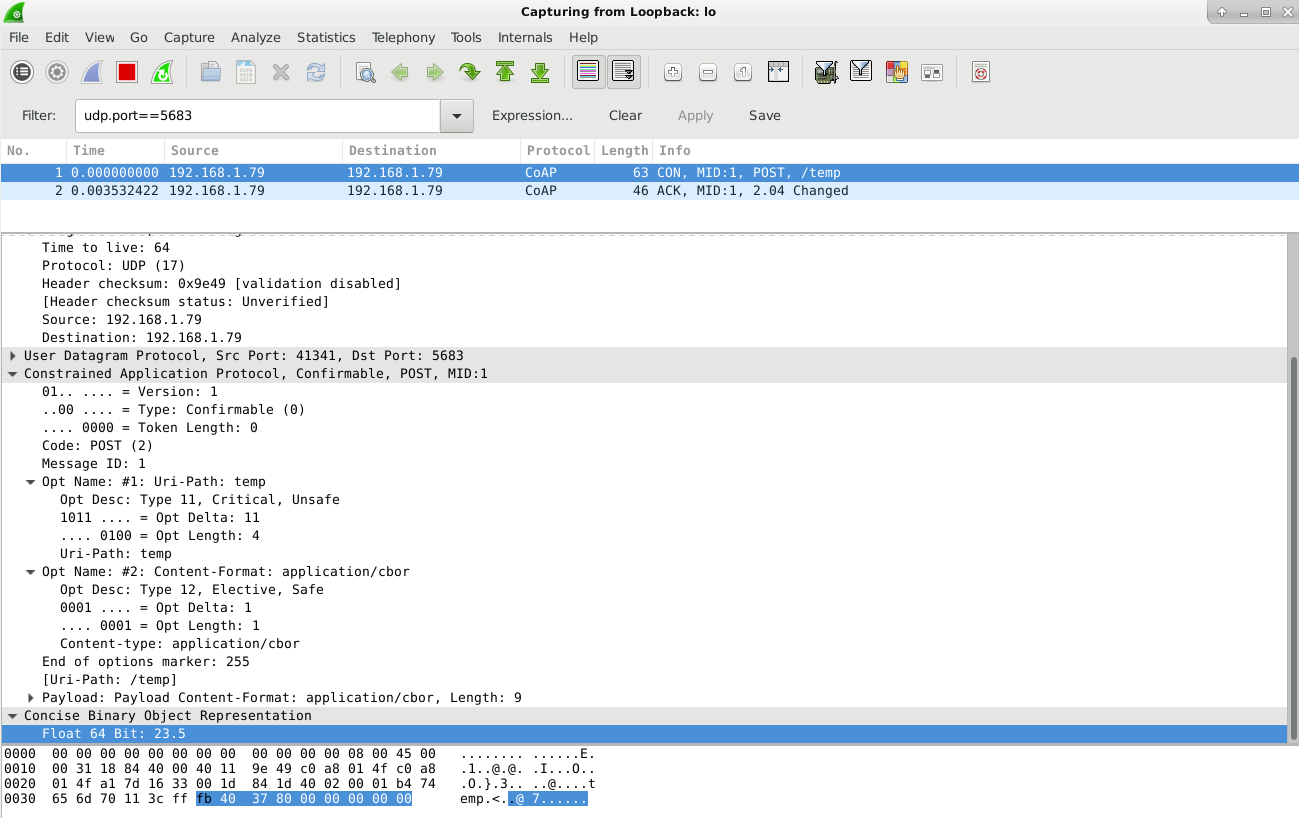
\includegraphics[width=1\columnwidth]{Pictures/aiocoap-ws.png}}
\caption{Trafic complet lié au POST}
\label{fig-post2-ws}
\end{figure}

\Question{Réponse}
{Que reçoit-on en réponse à la requête POST ?

 \begin{itemize}[label=$\circ$]
   \item \Wrong{un message ACK}
   \item \Wrong{le statut 2.00.}
   \item \Correct{le statut 2.04 CHANGED.}
   \item \Wrong{rien.}
\end{itemize}
 }
{
A chaque requête on reçoit une notification REST indiquant que la ressource a été modifiée. 
}

\Question{Réponse}
{Modifiez le programme client pour indiquer un content-format JSON. Quelle notification obtenez-vous ?


 \begin{itemize}[label=$\circ$]
   \item \Wrong{un message RST}
   \item \Wrong{le statut 4.04 NOT FOUND.}
   \item \Correct{le statut 2.15.}
   \item \Wrong{le statut 5.00.}
\end{itemize}
 }
{
Si vous avez 5.00 c'est qu'il y a une erreur dans votre programme coté serveur. La notification pour un format inconnu est 4.15 (Unsupported Content-Format)
}

\subsection{No Response}
Que l'on utilise le type CONfirmable ou NON confirmable, le serveur va envoyer une notification : 
\begin{itemize}
\item 2.xx quand tout se passe bien, et
\item 4.xx ou 5.xx quand le client ou le serveur a commis une erreur.
\end{itemize}

Si un capteur veut utiliser CoAP sur un réseau LPWAN, à chaque POST qu'il va envoyer sur la voie montante (uplink), il va récupérer un acquittement dans la voie descendante (downlink). Or, on a vu que l'on devait ménager cette dernière qui pouvait être sujette à saturation ou à facturation. 

L'option \Index{No response} définie dans le RFC 7967 permet à un client d'informer le serveur qu'il ne souhaite pas recevoir de notifications lors d'un POST ou d'un PUT.  La valeur de l'option est 258 et elle est suivie d'un octet contenant un bitmap qui va indiquer quel type de notification va être émis :
\begin{itemize}
    \item si le deuxième bit à partir de la droite est mis à 1, le client ne veut pas recevoir les notifications de type 2.xx ;
    \item si le quatrième bit à partir de la droite est mis à 1, le client ne veut pas recevoir les notifications de type 4.xx ;
    \item si le cinquième bit à partir de la droite est mis à 1, le client ne veut pas recevoir les notifications de type 5.xx.
\end{itemize}

Par exemple, en mettant la valeur \texttt{0x02} dans cette option, le client ne reçoit pas les acquittements positifs mais uniquement les erreurs 4.xx et 5.xx. En mettant la valeur \texttt{0b00011010} (0x1a, 26), le serveur sera complètement silencieux.

Le programme \pprog{coap\_post\_temp4.py}{pycom} ajoute cette option et le type du message CoAP a été fixé à NON confirmable. Cependant, le chemin d'URI n'est pas connu du serveur.  On voit que le serveur retourne un message d'erreur. Si en revanche le POST se déroule correctement, seul le client émet une donnée et le serveur reste silencieux.

\pycomlst[firstline=15,lastline=21, firstnumber=15]{coap\_post\_temp4.py}

\section{Chaîne complète de remonté de mesures}

 \begin{wrapfigure}{r}{3cm}
\Youtube{https://youtu.be/TFeeSEqGhPk}
\end{wrapfigure}


Voilà ! nous pouvons mettre les différents concepts ensemble pour construire une chaîne complète de remontée d'informations sur la température, l'humidité et la pression.

         \vspace{1em}

Côté capteur, nous allons~:

\begin{itemize}
    \item si le BME280 est présent, récupérer directement les données. Sinon, nous allons utiliser les mesures virtuelles. Nous allons également définir le protocole réseau : WiFi, Sigfox, LoRaWAN ;
    \item si nous utilisons un réseau LoRaWAN, nous devons mettre en place un programme relais pour transmettre les données vers le serveur CoAP ;
\end{itemize}

Le serveur CoAP doit pouvoir envoyer les données au serveur Beebotte pour affichage.

         \vspace{1em}

Le message CoAP va être configuré de la manière suivante :
\begin{itemize}
\item type = NON pour éviter les acquittements des messages CoAP ;
\item l'option No Response à 2 pour éviter les notifications REST positives. On garde sur la voie descendante les notifications d'erreurs pour permettre au capteur d'arrêter de transmettre ou d'augmenter sa période d'émission si le serveur n'est pas capable de traiter les données. Cela permettra de limiter l'usage du spectre et de préserver l'énergie des capteurs ;
\item 3 chemins d'URI pour les 3 valeurs mesurées ;
\item le codage en CBOR des séries temporelles.
\end{itemize}

         \vspace{1em}

Il reste un point à traiter car avec la limitation à 12 octets des trames \Index{Sigfox}, il est impossible de transmettre des données si on utilise CoAP. En effet, l'en-tête CoAP va contenir :
\begin{itemize}
\item 4 octets pour l'en-tête obligatoire ;
\item 0 octets de Token ;
\item 2 octets au minimum pour l'option URI-path si on réduit à un caractère le chemin ; par exemple \texttt{T}, \texttt{H}, \texttt{P} pour représenter la température, l'humidité et la pression ;
\item 2 octets pour l'option \Index{Content-format} indispensable pour indiquer que l'on transporte du CBOR ;
\item 3 octets pour l'option \Index{No-response}, également indispensable pour indiquer que l'on ne veut surtout pas d'acquittement (Sigfox les limitant à 4 par jour).
\end{itemize}
Soit, au total 11 octets. Il n'en reste plus qu'un. Si la température dépasse les 23 °C, l'information ne sera pas transportable.

\section{SCHC}

\acl{SCHC}, défini dans le \rfc{8724}, donne l'acronyme SCHC que l'on prononce Chic. SCHC propose un mécanisme de compression générique des en-têtes. SCHC se base sur un contexte commun à l'émetteur et au récepteur qui va permettre d'éliminer les informations connues dans le message et de ne transmettre que les données qui ne peuvent pas être prédéterminées.

         \vspace{1em}

Nous allons mettre en œuvre une version simplifiée. Dans le message CoAP, nous avons besoin du champ Message ID qui va servir à éliminer les doublons qui pourraient apparaître dans le réseau. Les serveurs CoAP gardent en mémoire les informations concernant les Messages ID pendant 5 minutes. Donc, la numérotation des messages doit permettre des périodes plus longues avant de réutiliser les mêmes valeurs. Nous allons également transporter 3 types de ressources : \texttt{/temperature}, \texttt{/humidity} et \texttt{/pressure}.

         \vspace{1em}

On peut donc construire manuellement un en-tête SCHC avec les champs suivants :
\begin{itemize}
\item 2 bits pour numéroter les règles de compression. Dans notre cas, nous n'utiliserons que la règle 00 ;
\item 4 bits pour numéroter les messages ID, ce qui donne 15 valeurs possibles de 1 à 15. Au pire, il faudrait émettre plus de 3 trames par minutes pour que le serveur CoAP traite deux trames différentes comme des doublons ;
\item 2 bits pour désigner les chemins d'URI ; 3 seront utilisés.
\end{itemize}

         \vspace{1em}

Cela fait appel à plusieurs techniques de compression définies par SCHC :
\begin{itemize}
\item \textit{\Index{not\_sent}}~: la valeur d'un champ n'est pas envoyée sur le réseau car elle se trouve dans les règles. Cela s'appliquera à la plupart des champs ;
\item \textit{\Index{Least Significant Bit}} : on n'envoie que les bits de poids faible. Cela s'applique au champ Message ID duquel on ne va transmettre que les 4 bits de poids faible ;
\item \textit{\Index{Matching\_sent}} : au lieu d'envoyer la valeur, on va envoyer un index sur un tableau commun. Cela s'applique à Uri-path où l'on enverra 00 pour l'élément temperature, 01 pour l'élément pressure, et 10 pour élément humidity. 
\end{itemize}

         \vspace{1em}

\subsection{Emission côté client}

La compression très simplifiée que nous allons effectuer se fera au moment de l'envoi des données pour Sigfox dans le programme \lprog{coap\_full\_sensor.py}{pycom}.

\pycomlst[firstline=174,lastline=198, firstnumber=174]{coap\_full\_sensor.py}

Dans le cas de Sigfox, on prend l'index en cherchant l'élément dans le tableau (ligne 183). On construit ensuite l'octet SCHC en ajoutant un numéro de règle (ligne 185) et les 4 bits de poids faible du champ Message ID qui va donc varier de 1 à 15 (ligne 186). Puis, l'on concatène les données CBOR a envoyer (ligne 193).

         \vspace{1em}

Pour les autres technologies de transmission, l'en-tête CoAP est construite avec les fonctions du module CoAP.py.

\pycomnxt[firstline=200,lastline=208, firstnumber=200]{coap\_full\_sensor.py}

L'envoi de la trame se fait avec la fonction \texttt{send\_ack}. Comme le message est de type NON, cette fonction n'attend pas de réponse après l'émission des données.

\subsection{Réception côté serveur}

Si les données émises par \lprog{coap\_full\_sensor.py}{pycom} passent par un réseau LPWAN, le programme \pprog{generic\_coap\_relay.py}{plido-tp4} va servir d'intermédiaire pour les envoyer au serveur CoAP. Le programme est presque identique à celui que nous avions utilisé pour transmettre dans la session précédente. Les seules différences sont~:
\begin{itemize}
    \item les numéros de ports utilisés : 5683 au lieu de 33033~;
    \item l'ajout de la décompression SCHC pour les données venant de Sigfox.
\end{itemize}

\pythonlst[firstline=69,lastline=89, firstnumber=69]{generic\_coap\_relay.py}

Pour reconstruire l'en-tête CoAP, SCHC se base sur des règles pour rendre le traitement indépendant des champs employés par le protocole. Mais ici, pour faire plus simple, nous utilisons le module Message d'\Index{aoicoap} pour reconstituer le message CoAP.

Dans un premier temps, on extrait du premier octet la valeur du champ message ID et l'index des URI (ligne 72 à 74) puis, à partir de ces valeurs et de celles connues à l'avance, le message CoAP est reconstitué.

         \vspace{1em}

Dans tous les cas, la fonction \texttt{forward\_data} est utilisée. Elle retourne la réponse du serveur CoAP qui est renvoyée au réseau LPWAN suivant les principes que nous avions vus lors de la session précédente. Nous ne l'avons pas mis en œuvre pour Sigfox pour éviter une erreur vu que 4 messages par jours sont autorisés.

\subsection{serveur CoAP}

Finalement, le programme \pprog{coap\_server.py}{plido-tp4} a été étendu à différents chemins d'URI pour traiter les différentes ressources que vont nous envoyer les capteurs. Et dans le traitement de la ressource, l'appel a la fonction to_bbt a été ajouté.

\section {Pistes d'améliorations}

Vous pouvez étendre cet ensemble de programmes. Voici quelques pistes d'amélioration :

\begin{itemize}

\item les capteurs envoient également leur mémoire disponible. Cela peut être utile pour détecter une fuite dans la mémoire ; par exemple quand une structure n'est jamais libérée. La structure CBOR est bien envoyée mais ni \texttt{coap\_server.py} ni Beebotte n'ont été configurés pour afficher ces valeurs. Vous pouvez donc l'intégrer dans la chaîne de traitement ;
\item le POST de la mémoire conduit à l'émission d'un message en downlink pour indiquer l'erreur 4.04. C'est une conséquence de l'utilisation de l'option CoAP \Index{no\_response} qui ne bloque que les notifications de type 2.xx. Vous pouvez modifier le module CoAP.py pour que la réponse soit traitée. Par exemple, en limitant à un envoi par jour de cette ressource ;
\item en plus de la mémoire, il peut être intéressant d'envoyer le niveau de la batterie. La page \href{https://forum.pycom.io/topic/1690/correct-formula-for-batt-monitoring-on-expansion-board}{Correct formula for BATT monitoring on expansion board | Pycom user forum}\footnote{https://forum.pycom.io/topic/1690/correct-formula-for-batt-monitoring-on-expansion-board} donne des indications pour récupérer le niveau de la batterie ;
\item finalement, nous n'avons pas réglé tous les problèmes d'interopérabilité. Si, par exemple, vous voulez envoyer toutes les heures un relevé de la mémoire libre et toutes les minutes la température, vous devez également modifier le programme \texttt{coap\_server.py}. Si ces paramètres sont transmis de manière optimale par le serveur, le programme \texttt{coap\_serveur} peut devenir complètement indépendant de la valeur mesurée.
\end{itemize}